% EN49 c11 | 原书 p.112–127（PDF 123–138） | 第 8 章 §8.1–8.3
\section{限制函子}

\subsection{Kn{\"o}rrer 周期性}

% ===== 原书 p.112 =====
在研究镜像对称之前，我们需要先理解定理 \ref{thm:6-1-16} 中 Kn{\"o}rrer 周期性等价所起的作用：

\begin{lemma}\label{lem:8-1-1}
Kn{\"o}rrer 周期性给出 dg 函子的交换图表：
\[
\begin{tikzcd}[column sep=3.4em, row sep=1.9em]
& \operatorname{Coh}_{\mathbb G_m}(\cK_X\times\mathbb A^1,s(x)yz) & \\
\operatorname{Coh}(Z) \arrow[ur] & & \operatorname{Coh}(\tilde Z) \arrow[ul] \\
& \operatorname{Coh}(D) \arrow[ul] \arrow[ur] &
\end{tikzcd}
\]
\end{lemma}

\transnote{易错预警：引理 \ref{lem:8-1-1} 的图表四边都没有标函子名，这是原书排版如此，并非漏标；各边函子在证明中逐一给出。}

\begin{proof}
下面两个映射由拉回-推前函子（pull-push functor）给出：$j_{D*}p_D^*$（其中 $p_D\colon\cK_X|_D\to D$，$j_D\colon\cK_X|_D\to Z$）与 $j_{\tilde D*}p_{\tilde D}^*$（其中 $p_{\tilde D}\colon D\times\mathbb A^1[-1]\to D$，$j_{\tilde D}\colon D\times\mathbb A^1[-1]\to\tilde Z$）。左上函子同样由 $j_{Z*}p_Z^*$ 给出（$p_Z$ 为投影 $Z\times\mathbb A^1\to\cK_X$，$j_Z$ 为包含 $Z\times\mathbb A^1\to\cK_X\times\mathbb A^1$）。右上函子是命题 \ref{prop:6-1-9} 与 \ref{prop:6-1-10} 中的等价链
\[
\operatorname{Coh}(\tilde Z)\to\operatorname{Coh}_{\mathbb G_m}(\tilde Z,0)\to\operatorname{Coh}_{\mathbb G_m}(\cK_X\times\mathbb A^1,s(x)yz),
\]
其中第二个也由拉回-推前函子 $j_{\tilde S*}p_{\tilde S}^*$ 给出。

% ===== 原书 p.113 =====
从命题 \ref{prop:6-1-9} 的证明中对第一个等价的显式描述可以检查：$X$ 上支撑在 $D$ 上、且作为 $z$-模自由的相干层，给出的矩阵分解同样支撑在 $D$ 上、并在 $z$ 变量上自由。最后，只需在仿射情形检查图表两边的复合
\[
j_{Z*}p_Z^*j_{D*}p_D^*=j_{Z*}(p_D\circ p_Z|_{\cK_X|_D})_*=j_{\hat D*}p_{\hat D}^*=j_{\tilde S*}p_{\tilde S}^*j_{\tilde D*}p_{\tilde D}^*,
\]
其中 $p_{\hat D}\colon\cK_X|_D\times\mathbb A^1\to D$，$j_{\hat D}\colon\cK_X|_D\times\mathbb A^1\to\cK_X\times\mathbb A^1$；这就说明图表交换。
\end{proof}

% ===== 原书 p.114 =====
\begin{figure}[htbp]
\centering
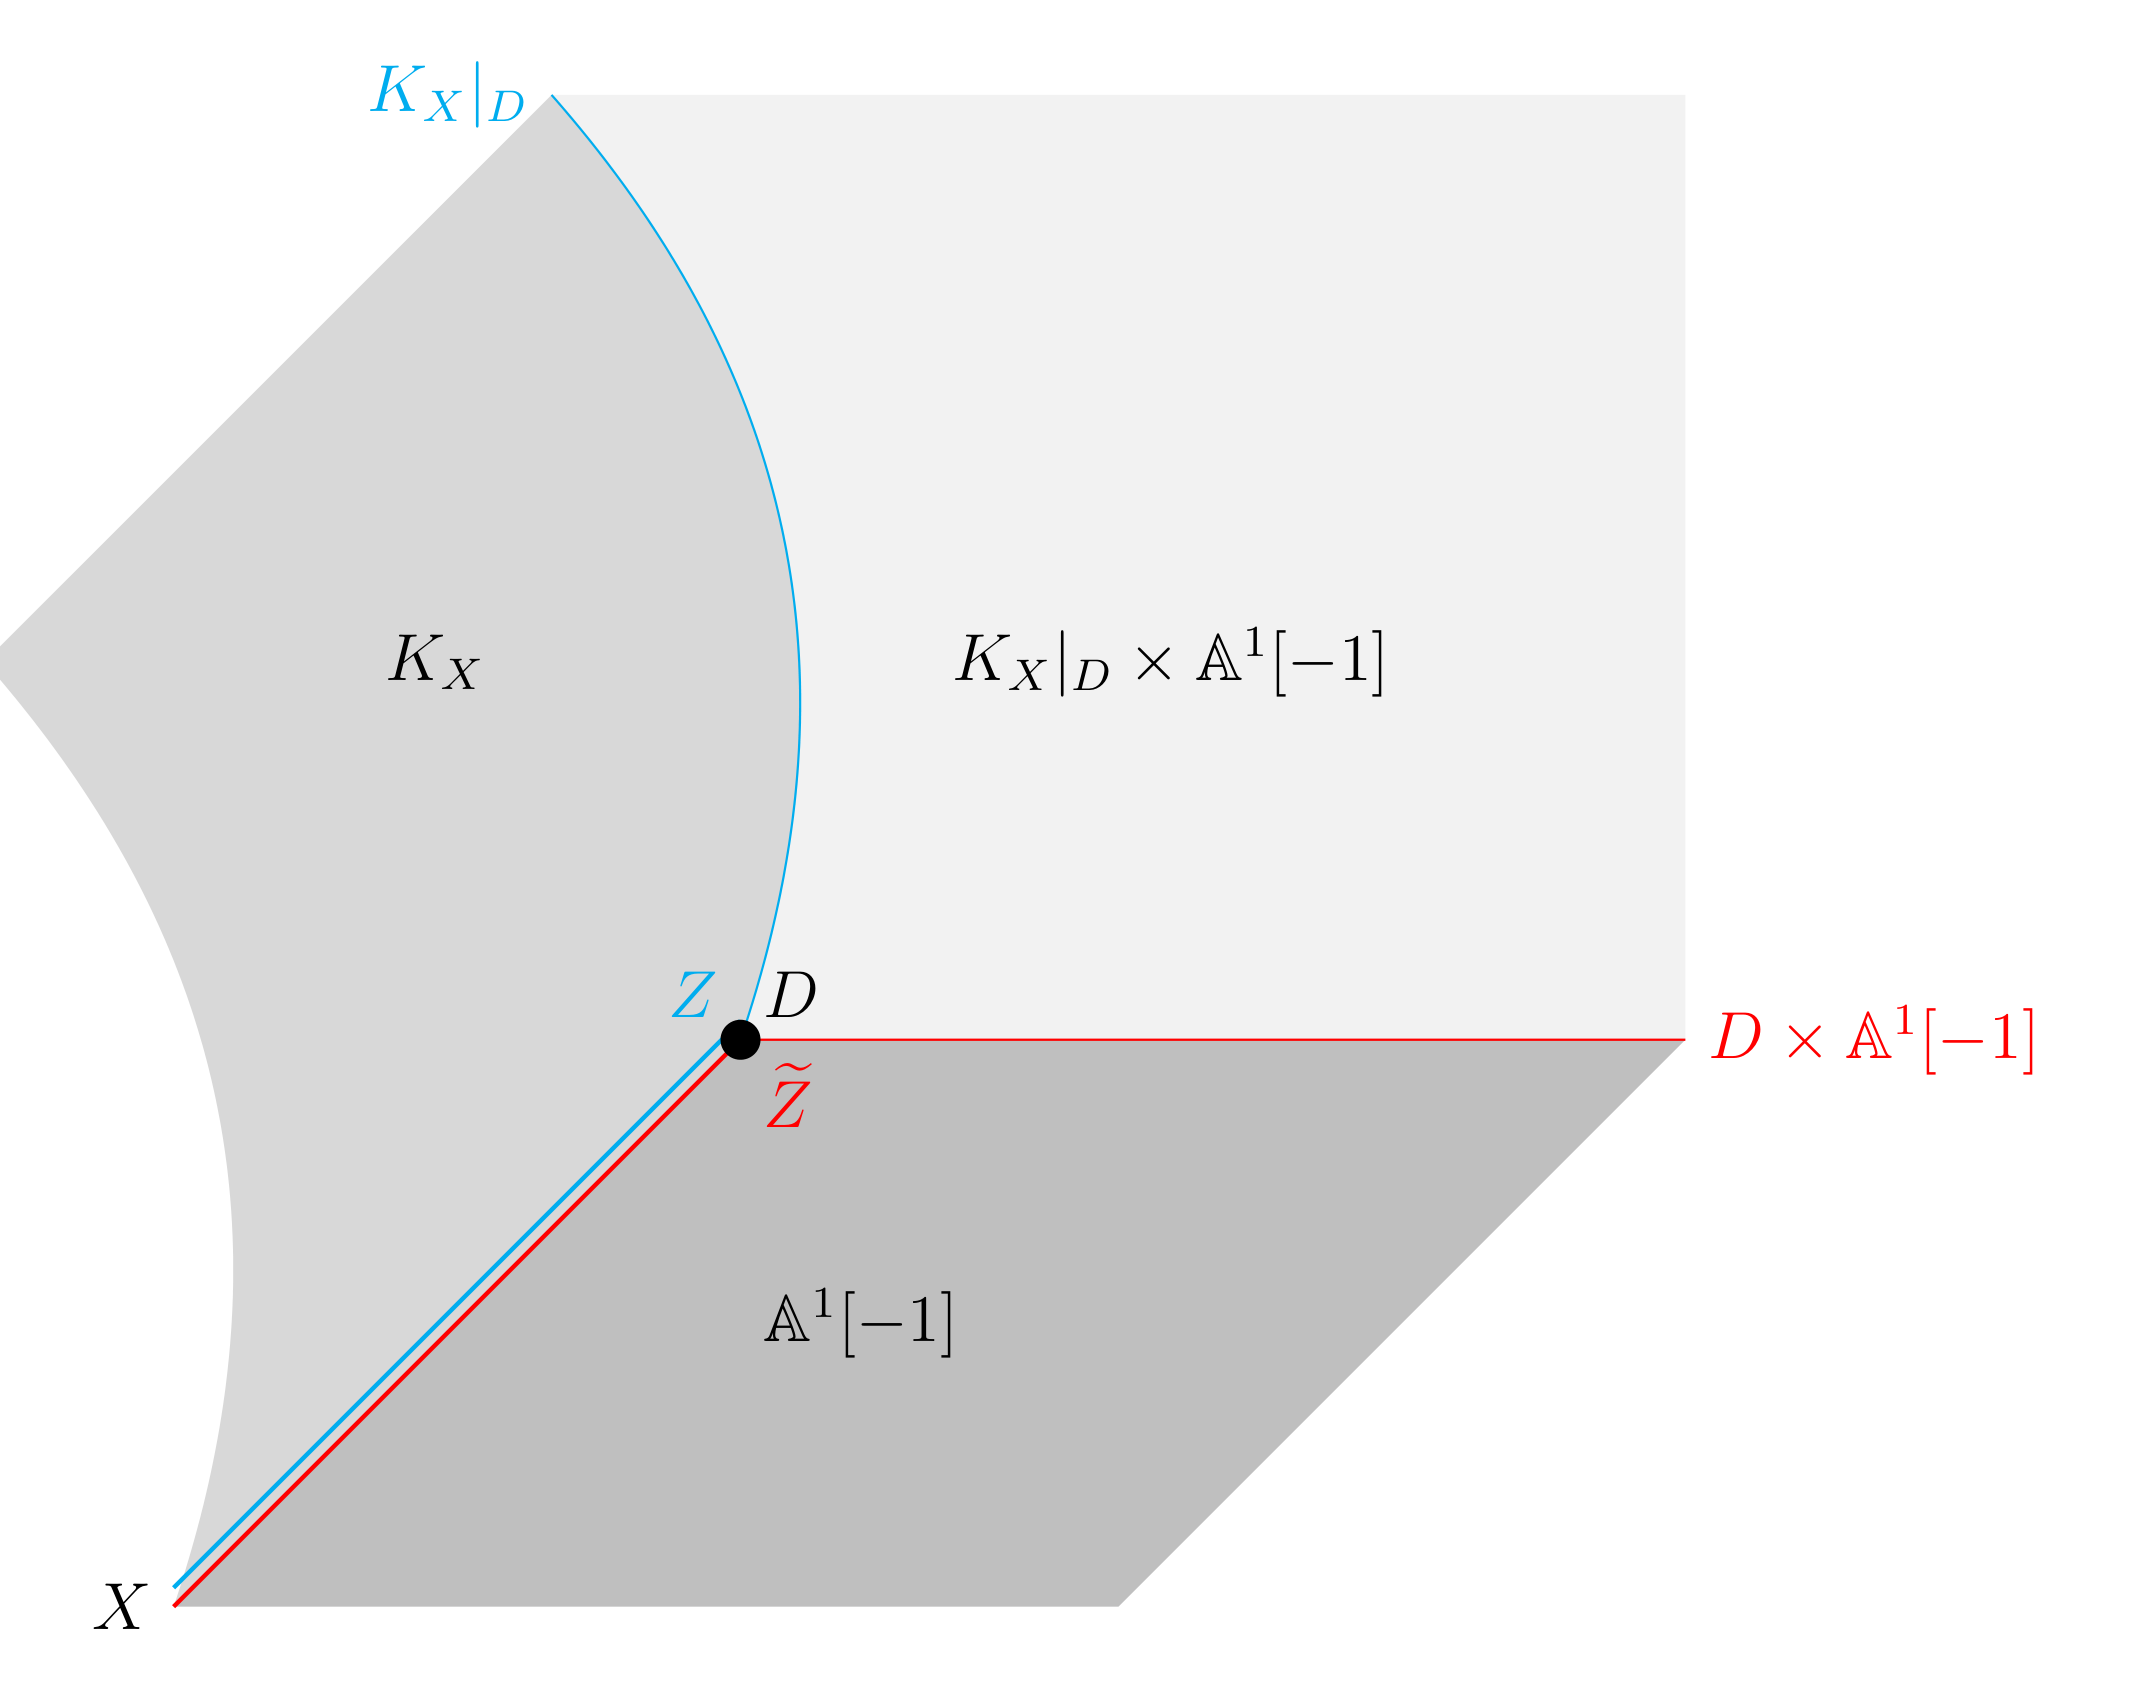
\includegraphics[width=0.66\textwidth]{figures/fig8_1.png}
\caption{$X=\mathbb A^1$ 时 $\cK_X\times\mathbb A^1[-1]$ 的示意图。}
\label{fig:8-1}
\end{figure}

\begin{lemma}\label{lem:8-1-2}
Kn{\"o}rrer 周期性给出 dg 函子的交换图表：
\[
\begin{tikzcd}[column sep=3.4em, row sep=1.9em]
& \operatorname{Coh}_{\mathbb G_m}(\cK_X\times\mathbb A^1,s(x)yz) & \\
\operatorname{Coh}(Z) \arrow[ur] & & \operatorname{Coh}(\tilde Z) \arrow[ul] \\
& \operatorname{Coh}(X) \arrow[ul, "{\pi_X^*[1]}"'] \arrow[ur, "i_{\tilde X*}"'] &
\end{tikzcd}
\]
\end{lemma}

\begin{proof}
设 $\mathcal E=\pi_X^*\mathcal F$ 是 $X$ 上局部自由层（locally free sheaf）$\mathcal F$ 的拉回，并记 $p_Z$ 为投影 $Z\times\mathbb A^1\to Z$。左上等价 $\operatorname{Coh}(Z)\to\operatorname{Coh}_{\mathbb G_m}(\cK_X\times\mathbb C,s(x)yz)$ 把 $\mathcal E$ 送到 $p_Z^*\mathcal E$ 沿包含 $j_Z\colon Z\times\mathbb A^1\to\cK_X\times\mathbb A^1$ 的推前。注意

% ===== 原书 p.115 =====
$\hat Z$ 上存在相干层的正合列
\[
0\to\OO_{Z\times\mathbb A^1}\to\OO_{\hat Z}\to\OO_{\cK_X\times\{0\}}\to0,
\]
它由函数的限制 $\OO_{\hat Z}\to\OO_{\cK_X\times\{0\}}$ 给出（这里没有正规丛（normal bundle）修正，因为 $\cK_X\times\{0\}=\{z=0\}$ 是平凡线丛的一个截面的零点轨迹（zero-locus））。对投影 $p_{\hat Z}\colon\hat Z\to X$，拉回 $p_{\hat Z}^*\mathcal F$ 是局部自由层。把它与上述正合列作张量积，得到正合三角
\[
\begin{tikzcd}[column sep=4.2em, row sep=1.5em]
j_{Z*}p_Z^*\mathcal E \arrow[rr] & & p_{\hat Z}^*\mathcal F \arrow[dl] \\
& \OO_{\cK_X\times\{0\}}\otimes p_{\hat Z}^*\mathcal F \arrow[ul, "+1"'] &
\end{tikzcd}
\]
\transnote{易错预警：正合三角回边上的 $+1$ 表示平移（shift），不是符号；三条边依次为 $j_{Z*}p_Z^*\mathcal E$、$p_{\hat Z}^*\mathcal F$、$\OO_{\cK_X\times\{0\}}\otimes p_{\hat Z}^*\mathcal F$。}
注意：过渡到商范畴 $\operatorname{Sing}(\hat Z)$ 会把所有局部自由层送到零。于是 $j_{Z*}p_Z^*\mathcal E[1]$ 在 $\operatorname{Sing}(\hat Z)$ 中等价于层 $\OO_{\cK_X\times\{0\}}\otimes p_{\hat Z}^*\mathcal F$。而后者恰好是 $i_{\tilde X*}\mathcal E|_X$ 在 $\operatorname{Coh}(\cK_X\times\mathbb C)$ 中的像，取像的函子为 $j_{\tilde Z*}p_{\tilde Z}^*\colon\operatorname{Coh}(\tilde Z)\to\operatorname{Coh}_{\mathbb G_m}(\cK_X\times\mathbb C,s(x)yz)$。由于 $X$ 光滑，该图表对所有相干层也交换。

接下来需要检查图表在态射层面交换。不妨设 $h\colon\mathcal F\to\mathcal G$ 是 $X$ 上局部自由层之间的态射。沿左手边把箭头走一遍，得到矩阵分解的态射
\[
\tilde h\colon\OO_{Z\times\mathbb A^1}\otimes p_{\hat Z}^*\mathcal F[1]\to\OO_{Z\times\mathbb A^1}\otimes p_{\hat Z}^*\mathcal G[1];
\]
而在右手边得到态射
\[
\tilde h\colon\OO_{\cK_X\times\{0\}}\otimes p_{\hat Z}^*\mathcal F\to\OO_{\cK_X\times\{0\}}\otimes p_{\hat Z}^*\mathcal G,
\]
其中 $\tilde h(x,y,z)=h(x)$。在我们选定的同构 $\OO_{\cK_X\times\{0\}}\cong\OO_{Z\times\mathbb A^1}[1]$ 之下，两者互相等同。
\end{proof}

\begin{definition}\label{def:8-1-3}
函子 $q\colon\overline{\operatorname{Coh}}(Z)\to\overline{\operatorname{Sing}}(Z)$ 是 dg 商函子（dg quotient functor），它把所有完美复形（perfect complex）送到零。
\end{definition}

% ===== 原书 p.116 =====
\begin{definition}\label{def:8-1-4}
局部化函子（localization functor）loc 把 $\overline{\operatorname{Coh}}(D\times\C^\times[-1])$ 映射到 $\overline{\operatorname{Coh}}(D)$：它局部化于一个 2 次自然变换，该自然变换由 $\C[z^{\pm1}]\cong\End(\OO_{\C^\times[-1]})$ 的生成元 $z$ 的作用给出（见引理 \ref{lem:koszul-duality}）。
\end{definition}

可与命题 \ref{prop:8-2-2} 对照。注意这两个函子（按这里的呈现方式）都只是 $\Z/2$-分次的。

\transnote{易错预警：本节起大量范畴带上横线（如 $\overline{\operatorname{Coh}}$），它表示同调分次的模 2 约化，不是复共轭或闭包。}

\begin{proposition}\label{prop:8-1-5}
在定理 \ref{thm:6-1-16} 中的 Kn{\"o}rrer 等价之下，我们有 $\C((\beta))$-线性 dg 范畴的交换图表：
\[
\begin{tikzcd}[column sep=3.0em, row sep=1.7em]
\overline{\operatorname{Coh}}(\tilde Z) \arrow[r, "j_{\tilde D}^*"] \arrow[d, "{\sim}"'] & \overline{\operatorname{Coh}}(D\times\C^\times[-1]) \arrow[r, "loc"] & \overline{\operatorname{Coh}}(D) \arrow[dd, "{\sim}"'] \\
\overline{\operatorname{Coh}}_{\mathbb G_m}(\cK_X\times\mathbb A^1,s(x)yz) & & \\
\overline{\operatorname{Coh}}(Z) \arrow[u, "{\sim}"'] \arrow[rr, "q"'] & & \overline{\operatorname{Sing}}(Z)
\end{tikzcd}
\]
\end{proposition}

\begin{proof}
设 $\mathcal E$ 是 $Z$ 上的局部自由层：它可以由某个 $X$ 上的局部自由层拉回得到。于是在引理 \ref{lem:8-1-2} 的等价链 $\operatorname{Coh}(Z)\to\operatorname{Coh}(\tilde Z)$ 之下，$\mathcal E$ 被送到 $i_{\tilde X*}\mathcal E|_X[-1]$，而后者在拉回到 $D\times\C^\times$ 的映射下显然被送到零。因此沿图表两个方向走，都把 $Z$ 上所有局部自由层送到零。

% ===== 原书 p.117 =====
第二部分的论证如下。由引理 \ref{lem:6-1-7}，$\C((\beta))$-线性等价 $\overline{\operatorname{Coh}}(D)\to\overline{\operatorname{Sing}}(Z)$ 通过商映射 $q$ 分解；因此 $q$ 在那些经由 $j_{D*}p_D^*$ 来自 $D$ 的层上是等价（这里 $p_D\colon\cK_X|_D\to D$、$j_D\colon\cK_X|_D\to Z$ 分别为投影与包含）。于是设 $\mathcal F$ 是 $Z$ 上支撑在 $\cK_X|_D$ 上的相干层，且经由 $\mathcal F=j_{D*}p_D^*\mathcal F_D$ 来自 $D$。由引理 \ref{lem:8-1-1}，这个层被送到 $\operatorname{Coh}(\tilde Z)$ 中的层 $\tilde{\mathcal F}$，其中 $\tilde{\mathcal F}=j_{\tilde D*}p_{\tilde D}^*\mathcal F_D$。注意：顶行的复合 $\operatorname{Coh}(\tilde Z)\to\operatorname{Coh}(D)$ 把 $\tilde{\mathcal F}$ 送到 $\mathcal F_D$。在引理 \ref{lem:6-1-7} 的等价之下，$\mathcal F_D$ 被送到矩阵分解 $F$：
\[
F_0=\bigoplus_{n\in\Z}i_{Z*}j_{D*}p_D^*\cF_D^{2n}(\chi^{-n}),\qquad
F_1=\bigoplus_{m\in\Z}i_{Z*}j_{D*}p_D^*\cF_D^{2m+1}(\chi^{-m}),
\]
它位于 $\operatorname{Coh}_{\mathbb G_m}(\cK_X,s(x)y)$ 中。另一方面，$\mathcal F$ 在 $\operatorname{Coh}(Z)$ 中被送到层 $i_{Z*}\mathcal F$，后者同样给出 $\operatorname{Coh}_{\mathbb G_m}(\cK_X,s(x)y)$ 中的一个矩阵分解。作为 $\Z/2$-分次的矩阵分解，这与上面的 $F$ 相同，因为 $\mathcal F=j_{D*}p_D^*\mathcal F_D$。

类似地，设 $h_D\colon\mathcal F_D\to\mathcal G_D$ 是 $D$ 上相干层复形的 $k$ 次态射；由引理 \ref{lem:6-1-7}，$\tilde Z$ 上对应的相干层态射 $\tilde h\colon\tilde{\mathcal F}\to\tilde{\mathcal G}$ 也以 $j_{\tilde D*}p_{\tilde D}^*(h_D)$ 的形式出现，次数同为 $k$。由于 $\tilde h$ 与 $z$ 无关，在局部化函子之下 $\tilde h$ 直接被送到 $\Hom^{k\,(\mathrm{mod}\,2)}(\mathcal F_D,\mathcal G_D)$ 中的 $h_D$。这说明：当态射的次数模 2 计时，图表交换。
\end{proof}

\subsection{镜像对称}

% ===== 原书 p.118 =====
首先，我们可以给出猜想 \ref{conj:aur-funct} 第 3 部分的一个版本：

\begin{theorem}\label{thm:8-2-1}
$\cW_0((\C^*)^n\setminus H)$ 与 $\operatorname{Coh}(Z)$ 之间存在镜像对称等价：它由定理 \ref{thm:7-2-4} 中 $\cW_0((\C^*)^n\setminus H)$ 与 $\operatorname{Coh}(\tilde Z)$ 的镜像等价，复合定理 \ref{thm:6-1-16} 中的等价链 $\operatorname{Coh}(\tilde Z)\to\operatorname{Coh}(Z)$ 得到。

在此等价之下，函子 $\alpha_\infty\colon\cW((\C^*)^n,f)\to\cW_0((\C^*)^n\setminus H)$ 镜像于 $\pi_X^*[1]\colon\operatorname{Coh}(X)\to\operatorname{Coh}(Z)$。
\end{theorem}

\transnote{易错预警：定理 \ref{thm:8-2-1} 的等价不是一步给出的，而是「定理 \ref{thm:7-2-4} 的等价」与「定理 \ref{thm:6-1-16} 的等价链」的复合；函子 $\alpha_\infty$ 的像 $\pi_X^*[1]$ 也须在这一复合下理解。}

\begin{proof}
应用引理 \ref{lem:8-1-2} 即得。
\end{proof}

来自 [Aur18, §4] 的限制函子 $\rho\colon\cW_0((\C^*)^n\setminus H)\to\cW(H)$ 在某种意义上是唯一的，因此我们在这里花些篇幅描述它。这样的函子甚至是否存在，远非显而易见：分次的选择尤其重要。

限制函子定义的第一步由 Viterbo 限制 [GPS19, §11.1] 给出：从 $(\C^*)^n\setminus H$ 限制到命题 \ref{prop:7-1-1} 第 (1) 部分的子区域 $H\times\C^*$。这一步可以在 $\Z$-分次范畴的层面上完成。此外，由于 $H\times\C^*$ 是 Weinstein 流形，Viterbo 限制函子可以定义在扭复形范畴上 [GPS19, (11.5)]。

由 [GPS19, Corollary 1.18] 的 K{\"u}nneth 定理，wrapped Fukaya 范畴 $\cW(H\times\C^*(2))$ 由形如 $\ell\times\R_{>0}$ 的对象的（柱化，cylindrization）生成，其中 $\ell$ 是 $H$ 中的拉格朗日量。在对象层面，函子 $\rho$ 应当把 $\ell\times\R_{>0}$ 送到 $\ell$：然而它在态射层面是否良定义并不清楚，因为没有可选取的参考纤维 $H\times\{p\}$，用来在 $H\times\C^*$ 中取两个拉格朗日量的相交。可是，如果我们使用 $H\times\C^*$ 上的 0-分次，它就会良定义：这镜像于代数几何中取 $\mathbb A^1[-1]$ 里「一般点」（generic point）上纤维的构造。

\transnote{背景直觉：没有参考纤维 $H\times\{p\}$，就无法在态射层面取两个拉格朗日量的相交；0-分次相当于用 $\mathbb A^1[-1]$ 上「一般点」的纤维代替这个缺失的参考纤维。}

为说明这一点，我们从最简单的例子开始，其中 $H$ 只是一个点：

% ===== 原书 p.119 =====
\begin{proposition}\label{prop:8-2-2}
当 $|z|=2$ 时，存在从有限生成 $\C[z^{\pm1}]$-模范畴到 $\Z/2$-分次有限维 $\C$ 向量空间范畴的自然函子，它把 $\C[z^{\pm}]$ 送到 0 次的 $\C$。此外，这给出从 $\C[z^{\pm1}]$-模的带分次 dg 范畴（模上带有额外的 $\Z$-分次，且 $z$ 的次数为 0）到 $\C$ 向量空间的分次 $\C((\beta))$-周期 dg 范畴的分次函子。
\end{proposition}

\transnote{易错预警：「$|z|=2$」指 $z$ 作为 2 次映射把分次提高 2，不是 $z$ 的模长；正因如此才能按奇偶取 $F^{2k}$ 与 $F^{2k+1}$。}

\begin{proof}
给定有限生成 $\C[z^{\pm1}]$-模 $F$，它对应于一个有限维 $\C$ 向量空间序列 $F^\bullet$，连同 2 次映射 $z\colon F^k\to F^{k+2}$。于是可以如下定义 $\rho(F)$：对任意 $k\in\Z$，令 $V_0=F^{2k}$、$V_1=F^{2k+1}$。重要的是：给定 $\C[z^{\pm1}]$-模的态射 $f\colon F\to G$，即与 $z$ 交换的线性映射 $f^\bullet\colon F^\bullet\to G^\bullet$，我们通过 $f^0=f^{2k}\colon F^{2k}\to G^{2k}$ 与 $f^1=f^{2k+1}\colon F^{2k+1}\to G^{2k+1}$ 得到态射 $\rho(F)\to\rho(G)$。重要的是：这个定义与 $k\in\Z$ 的选取无关，并给出从有限生成 $\C[z^{\pm1}]$-模到 $\Z/2$-分次 $\C$ 向量空间的函子。
\end{proof}

注意：若改取 $z$ 的次数为 0，则不存在这样的构造：给定以次数 0 的变量 $z$ 写成的 Laurent 多项式，只挑出其中一个系数并不能定义函子。

在一般情形下，$\cW(H\times\C^*(2))$ 中两个对象 $L_1,L_2$ 之间的态射总带有 $\C[z^{\pm1}]$-作用：若 $L_1=\ell_1\times\R_{>0}$、$L_2=\ell_2\times\R_{>0}$，则态射由
\[
\Hom(L_1,L_2)\cong\Hom_{\cW(H)}(\ell_1,\ell_2)\otimes_\C\C[z^{\pm1}]
\]
给出，它带有显然的 $\C[z^{\pm1}]$-作用。给定 $L_1$ 与 $L_2$ 之间的态射 $p$，我们有映射
\[
\Hom^{2k}_{\cW(H\times\C^*(2))}(L_1,L_2)\xrightarrow{\ \sim\ }\Hom^{0}_{\cW(H\times\C^*(2))}(L_1,L_2)\to\Hom^{\mathrm{even}}_{\cW(H)}(\ell_1,\ell_2),
\]
它把 $p$ 的 $2k$ 次部分送到 $z^{-k}p$。类似地，把

% ===== 原书 p.120 =====
$p$ 的 $2k+1$ 次部分送到 $z^{-k}p$，就得到映射
\[
\Hom^{2k+1}_{\cW(H\times\C^*(2))}(L_1,L_2)\xrightarrow{\ \sim\ }\Hom^{1}_{\cW(H\times\C^*(2))}(L_1,L_2)\to\Hom^{\mathrm{odd}}_{\cW(H)}(\ell_1,\ell_2),
\]
对任意 $k\in\Z$ 成立；容易验证它给出从 $\cW(H\times\C^*(2))$ 到 $\Z/2$-分次范畴 $\overline{\cW}(H)$ 的良定义函子。

更精确地说，按照 [Aur18]，我们可以在 $A_\infty$-模上形式地定义 $\rho$：沿包含函子 $i\colon\cW(H)\to\cW(H\times\C^*(2))$ 拉回，该包含把拉格朗日量 $\ell$ 送到 $\ell\times\R_{>0}$。注意这个构造用到了 $H$ 在 $(\C^*)^n$ 中的一个标架（framing）选取。给定 $\cW(H\times\C^*(2))$ 中的 $L$，拉回模 $i^*(L)$ 绝不能由 $\cW(H)$ 的某个对象表示，因为它的上同调支撑（cohomological support）无界。Auroux 的关键观察是：$\C[z^{\pm1}]$ 的作用给 $i^*(L)$ 诱导出一个 2-周期结构 [Aur18, p.17]，于是 $i^*(L)$ 可由 $\C((\beta))$-线性范畴 $\overline{\cW}(H)$ 中的对象表示，这里我们把分次模 2 约化。某种意义上，范畴 $\cW(H\times\C^*(2))$ 只是 $\cW(H)$ 的 2-周期化（2-periodization）。函子 $\rho$ 恰好对应于局部化 $\cW(H\times\C^*(2))\to\overline{\cW}(H)$，局部化于 2 次自然变换 $z\colon\id\to[2]$，该变换由绕 $0$ 旋转 $\C^*$ 给出 [Aur18, (4.3)]，从而得到 $\Z/2$-分次范畴。总结如下：

\begin{definition}\label{def:8-2-3}
限制函子 $\rho\colon\overline{\cW}_0((\C^*)^n\setminus H)\to\overline{\cW}(H)$ 的定义如下：先取到命题 \ref{prop:7-1-1} 第 (1) 部分中区域 $H\times\C^*$ 的 Viterbo 限制；再取局部化函子 $\overline{\cW}(H\times\C^*(2))\to\overline{\cW}(H)$，局部化于由 $\End_{\cW(\C^*(2))}(\R_{>0})\cong\C[z^{\pm1}]$ 的生成元 $z$ 的乘法给出的 2 次自然变换（见 [Aur18, (4.3)]）。
\end{definition}

\transnote{含糊点拨：局部化于 2 次自然变换会把同调分次 2-周期化，因此只剩下 $\Z/2$-分次；这正是 $\rho$ 不能写成 $\Z$-分次函子的原因。}

回忆我们用上横线表示 $A_\infty$ 范畴同调分次的模 2 约化：$\overline{\cW}_0((\C^*)^n\setminus H)$

% ===== 原书 p.121 =====
与 $\overline{\operatorname{Coh}}(Z)$。注意这个 $\rho$ 函子只是 $\C((\beta))$-线性 $A_\infty$ 范畴的函子，因为我们局部化于一个 2 次自然变换。

\begin{proposition}\label{prop:8-2-4}
在上述关于函数 $\tilde f_0$ 的镜像对称等价之下，从 $(\C^*)^n\setminus H$ 到 $H\times\C^*$ 的 Viterbo 限制镜像于从 $\tilde Z$ 到 $D\times\C^*[-1]$ 的拉回：也就是说，$A_\infty$ 范畴的如下图表交换：
\[
\begin{tikzcd}[column sep=3.6em, row sep=1.7em]
\cW_0((\C^*)^n\setminus H) \arrow[r] \arrow[d, "\mathrm{Vit}"'] & \operatorname{Coh}(\tilde Z) \arrow[d, "j_{\tilde D}^*"] \\
\cW(H\times\C^*(2)) \arrow[r] & \operatorname{Coh}(D\times\C^*[-1])
\end{tikzcd}
\]
\end{proposition}

\begin{proof}
这由 [GS21, Corollary 5.8] 推出。
\end{proof}

\transnote{易错预警：命题 \ref{prop:8-2-4} 的图表照原书不带横线，与定理 \ref{thm:8-2-5} 的带横线版本不同；这是原书的不一致，译文照录。}

\begin{theorem}\label{thm:8-2-5}
限制函子 $\rho\colon\overline{\cW}_0((\C^*)^n\setminus H)\to\overline{\cW}(H)$ 镜像于商函子 $q\colon\overline{\operatorname{Coh}}(Z)\to\overline{\operatorname{Sing}}(Z)$ 与 Kn{\"o}rrer 周期性等价 $\overline{\operatorname{Sing}}(Z)\to\overline{\operatorname{Coh}}(D)$ 的复合（作为 $\C((\beta))$-线性 $A_\infty$ 范畴的函子，见引理 \ref{lem:6-1-7}）；这里的镜像对应在定理 \ref{thm:8-2-1} 的镜像对称等价之下。
\end{theorem}

\begin{proof}
在下面的图表中，左上方的方块由命题 \ref{prop:8-2-4} 交换；右上方的方块显然也交换，因为我们局部化于同一个自然变换。剩下要证下方方块交换，这正是命题 \ref{prop:8-1-5}。
\end{proof}

% ===== 原书 p.122 =====
\[
\begin{tikzcd}[column sep=3.0em, row sep=1.7em]
\overline{\cW}_0((\C^*)^n\setminus H) \arrow[r, "\mathrm{Vit}"] \arrow[rr, bend left=24, "\rho"] \arrow[d, "{\sim}"'] & \overline{\cW}(H\times\C^*(2)) \arrow[r, "loc"] \arrow[d, "{\sim}"'] & \overline{\cW}(H) \arrow[d, "{\sim}"'] \\
\overline{\operatorname{Coh}}(\tilde Z) \arrow[r, "j_{\tilde D}^*"] \arrow[d, "{\sim}"'] & \overline{\operatorname{Coh}}(D\times\C^\times[-1]) \arrow[r, "loc"] & \overline{\operatorname{Coh}}(D) \arrow[dd, "{\sim}"'] \\
\overline{\operatorname{Coh}}_{\mathbb G_m}(\cK_X\times\mathbb A^1,s(x)yz) & & \\
\overline{\operatorname{Coh}}(Z) \arrow[u, "{\sim}"'] \arrow[rr, "q"'] & & \overline{\operatorname{Sing}}(Z)
\end{tikzcd}
\]

\subsection{整分次增强}

到目前为止我们看到：函子 $q$ 与 $\rho$ 在一个 $\Z/2$-分次的同调镜像对称等价之下对应，即在一个 $\C((\beta))$-线性范畴的等价之下对应。本节要说明：所涉及的范畴都带有一个辅助的 $\Z$-分次，并且 $q$ 与 $\rho$ 可以在分次 $\C((\beta))$-线性范畴的等价之下对应起来。

\begin{definition}\label{def:8-3-1}
我们引入如下术语：
\begin{itemize}
\item 我们把由「在 $\mathbb G_m$-作用下给 $\mathbb A^1$ 权（weight）1」而来的分次，连同 $(\C^*)^n\setminus H$ 上的形式 $\eta_0$，称为\textbf{0-分次（0-grading）}；我们把它看作范畴上底层的同调分次结构。
\item 我们把由「在 $\mathbb G_m$-作用下给 $\cK_X$ 的纤维权 1」而来的分次，连同 $(\C^*)^n\setminus H$ 上的形式 $\eta_\infty$，称为\textbf{$\infty$-分次（$\infty$-grading）}；我们把它看作范畴上的
\end{itemize}
\end{definition}

% ===== 原书 p.123 =====
额外 $\Z$-分次结构。

使用 $\infty$-分次，就在 $A_\infty$ 范畴 $\cW_{0,\infty}((\C^*)^n\setminus H)$ 与 $\operatorname{Coh}_{\mathbb G_m}(Z)$ 上得到（额外的）分次；把同调分次模 2 约化，便得到分次 $\C((\beta))$-线性 $A_\infty$ 范畴。我们仍用上横线表示同调分次的模 2 约化（reduction mod 2）：$\overline{\cW}_{0,\infty}((\C^*)^n\setminus H)$ 与 $\overline{\operatorname{Coh}}_{\mathbb G_m}(Z)$。

现在可以定义限制函子 $\rho\colon\overline{\cW}_{0,\infty}((\C^*)^n\setminus H)\to\overline{\cW}(H)$ 的分次版本，步骤如下：
\begin{itemize}
\item 先取到子区域 $H\times\C^*$ 的 Viterbo 限制（[GPS19] 中的定义可以按分次方式执行），其中 $H\times\C^*$ 带有从 $(\C^*)^n\setminus H$ 的行列式丛（determinant bundle）平凡化限制而来的平凡化；然后，
\item 取局部化 $\overline{\cW}_{0,\infty}(H\times\C^*)\to\overline{\cW}(H)$，局部化于乘以 2 次自然变换 $z$。由于在 $\infty$-分次下乘以 $z$ 的次数为 0，后一个函子由命题 \ref{prop:8-2-2} 是分次 $A_\infty$ 函子。
\end{itemize}
于是 $\rho$ 是分次 $\C((\beta))$-线性 $A_\infty$ 范畴之间的分次函子（graded functor）。

同样地，等变相干层（equivariant coherent sheaf）上的商映射 $q\colon\operatorname{Coh}_{\mathbb G_m}(Z)\to\operatorname{Sing}_{\mathbb G_m}(Z)$ 不保持同调分次，但保持由 $\mathbb G_m$-等变结构给出的分次（参引理 \ref{lem:6-1-7}），后者正是 $\infty$-分次。于是它给出分次 $\C((\beta))$-线性 dg 范畴的分次函子 $q\colon\overline{\operatorname{Coh}}_{\mathbb G_m}(Z)\to\overline{\operatorname{Sing}}_{\mathbb G_m}(Z)$（这里 $\operatorname{Sing}_{\mathbb G_m}(Z)$ 上的 $\C((\beta))$-线性结构来自定理 \ref{thm:zgraded-orlov} 中与矩阵分解范畴的等价）。

这样，$\rho$ 与 $q$ 都有提升为分次函子的版本。接下来我们要说明，它们在分次意义下于镜像对称之下对应。

% ===== 原书 p.124 =====
\begin{lemma}\label{lem:8-3-2}
分次 $A_\infty$ 范畴 $\cW_{0,\infty}((\C^*)^n,f)$ 与 $\operatorname{Coh}_{\mathbb G_m^2}(X,0)$ 之间存在镜像对称等价，连同交换图表
\[
\begin{tikzcd}[column sep=3.6em, row sep=1.7em]
\cW(H) \arrow[r] \arrow[d, "\cup"'] & \operatorname{Coh}(D) \arrow[d, "i_{D*}"] \\
\cW_{0,\infty}((\C^*)^n,f) \arrow[r] & \operatorname{Coh}_{\mathbb G_m^2}(X,0)
\end{tikzcd}
\]
其中竖直箭头是 [GS22] 的等价。
\end{lemma}

\transnote{易错预警：$\mathbb G_m^2$ 指两个 $\mathbb G_m$-作用的积，不是群 $\mathbb G_m$ 的平方；两个作用分别来自 $X$ 与 $\mathbb A^1$。}

\begin{proof}
这不过是一个观察：行列式丛在任意一般纤维 $H$ 上与在 $((\C^*)^n,f)$ 上的两个平凡化在相差同伦的意义下一致；再结合两个 $\mathbb G_m$-作用在 $X$ 上都平凡这一事实。前者可以从命题 \ref{prop:7-1-1} 与 \ref{prop:7-1-2} 的每个粘合呈现都不改变子扇形 $((\C^*)^n,f)$ 看出。
\end{proof}

\transnote{含糊点拨：原书此处作 “The former is can be seen”，系笔误；译文按「前者可以从……看出」处理。}

\begin{theorem}\label{thm:8-3-3}
分次 $A_\infty$ 范畴 $\cW_{0,\infty}((\C^*)^n\setminus H)$ 与 $\operatorname{Coh}_{\mathbb G_m^2}(\tilde S,0)$ 之间存在镜像对称等价。
\end{theorem}

\begin{proof}
检查 [GPS19] 的论证可以发现：命题 \ref{prop:7-1-1} 的扇形分解给出分次 $A_\infty$ 范畴的推出图表（参 [GPS19, p.26]）：
\[
\begin{tikzcd}[column sep=4.0em, row sep=1.7em]
\cW(H) \arrow[r, "\cup"] \arrow[d] & \cW_{0,\infty}((\C^*)^n,f) \arrow[d] \\
\cW_{0,\infty}(H\times\C^*,z) \arrow[r] & \cW_{0,\infty}((\C^*)^n\setminus H)
\end{tikzcd}
\]
\transnote{易错预警：定理 \ref{thm:8-3-3} 的推出图表中两个竖直箭头没有标函子名（与推论 \ref{cor:7-1-4} 同），它们是扇形包含给出的函子，并非漏标。}
\end{proof}

% ===== 原书 p.125 =====
我们把这一粘合图表与命题 \ref{prop:6-2-2} 的粘合图表作比较：
\[
\begin{tikzcd}[column sep=3.0em, row sep=1.7em]
& \operatorname{Coh}_{\mathbb G_m^2}(D,0) \arrow[rr, "\iota_{\tilde D*}"] \arrow[dd, "i_{D*}"', pos=0.1] & & \operatorname{Coh}_{\mathbb G_m^2}(D\times\mathbb A^1,0) \arrow[dd, "j_{\tilde D*}", pos=0.1] \\
\cW(H) \arrow[ur, "{\sim}"] \arrow[rr, "\cup", pos=0.3] \arrow[dd, "\cup"'] & & \cW_{0,\infty}(H\times\C^*,z) \arrow[ur, "{\sim}"] \arrow[dd] & \\
& \operatorname{Coh}_{\mathbb G_m^2}(X,0) \arrow[rr, "i_{\tilde X*}"'] & & \operatorname{Coh}_{\mathbb G_m^2}(\tilde S,0) \\
\cW_{0,\infty}((\C^*)^n,f) \arrow[ur, "{\sim}"] \arrow[rr, "\alpha_\infty"'] & & \cW_{0,\infty}((\C^*)^n\setminus H) \arrow[ur, "{\sim}"] &
\end{tikzcd}
\]
\transnote{含糊点拨：此图中左竖与横中两条箭头都标 $\cup$，但它们是两个不同的 cup 函子：一条 $\cW(H)\to\cW_{0,\infty}((\C^*)^n,f)$，另一条 $\cW(H)\to\cW_{0,\infty}(H\times\C^*,z)$。}
再借助引理 \ref{lem:8-3-2} 便得到所需的等价。

\begin{proposition}\label{prop:8-3-4}
我们有分次 $A_\infty$ 范畴的交换图表：
\[
\begin{tikzcd}[column sep=3.6em, row sep=1.7em]
\cW_{0,\infty}((\C^*)^n\setminus H) \arrow[r] \arrow[d, "\mathrm{Vit}"'] & \operatorname{Coh}_{\mathbb G_m}(\tilde Z) \arrow[d, "j_{\tilde D}^*"] \\
\cW_{0,\infty}(H\times\C^*) \arrow[r] & \operatorname{Coh}_{\mathbb G_m}(D\times\C^*[-1])
\end{tikzcd}
\]
\end{proposition}

\begin{proof}
检查 [GS21, Corollary 5.8] 与 [FLTZ12] 的论证可以发现，相应结果可以推广到分次 $A_\infty$ 范畴。
\end{proof}

分次 $A_\infty$ 范畴层面的同调镜像对称等价，特别地通过把分次模 2 忘掉，下降到分次 $\C((\beta))$-线性 $A_\infty$ 范畴的层面。

\transnote{背景直觉：整分次增强的意思是——先把分次结构本身做成数据（0-分次或 $\infty$-分次），再要求 $q$ 与 $\rho$ 在这个分次意义下对应；单纯的 $\Z/2$ 等价无法区分两种分次。}

\begin{proposition}\label{prop:8-3-5}
在定理 \ref{thm:6-2-1} 中的 Kn{\"o}rrer 等价之下，我们有分次 $\C((\beta))$-线性 dg 范畴的交换图表：
\[
\begin{tikzcd}[column sep=2.6em, row sep=1.6em]
\overline{\operatorname{Coh}}_{\mathbb G_m^2}(\tilde S,0) \arrow[r, "j_{\tilde D}^*"] \arrow[d, "{\sim}"'] & \overline{\operatorname{Coh}}_{\mathbb G_m^2}(D\times\C^\times,0) \arrow[r, "loc"] & \overline{\operatorname{Coh}}(D) \arrow[dd, "{\sim}"'] \\
\overline{\operatorname{Coh}}_{\mathbb G_m^2}(\cK_X\times\mathbb A^1,s(x)yz) & & \\
\overline{\operatorname{Coh}}_{\mathbb G_m^2}(Z,0) \arrow[u, "{\sim}"'] \arrow[rr, "q"'] & & \overline{\operatorname{Sing}}_{\mathbb G_m}(Z)
\end{tikzcd}
\]
其中 $\operatorname{Coh}_{\mathbb G_m^2}(Z,0)$ 按引理 \ref{lem:6-2-3} 与 $\operatorname{Coh}_{\mathbb G_m}(Z)$ 等同。
\end{proposition}

% ===== 原书 p.126 =====
\begin{proof}
我们检查命题 \ref{prop:8-1-5} 的证明。第一，容易看出引理 \ref{lem:8-1-1} 与 \ref{lem:8-1-2} 也推广到分次 dg 版本。于是和前面一样，沿图表两个方向走，都把 $Z$ 上所有局部自由等变相干层送到零。重要的是：引理 \ref{lem:6-1-7} 中经由 $\operatorname{Coh}_{\mathbb G_m}(Z)$ 分解的等价是分次 dg 函子。现在，左侧的竖直等价由定理 \ref{thm:6-2-1} 是分次 dg 等价；而顶部的箭头只是分次 $\C((\beta))$-线性 dg 函子，因为局部化把同调分次 2-周期化了。把这些观察与命题 \ref{prop:8-1-5} 的证明结合起来，即得结论。
\end{proof}

\begin{theorem}\label{thm:8-3-6}
限制函子 $\rho\colon\overline{\cW}_{0,\infty}((\C^*)^n\setminus H)\to\overline{\cW}(H)$ 镜像于商函子 $q\colon\overline{\operatorname{Coh}}_{\mathbb G_m}(Z)\to\overline{\operatorname{Sing}}_{\mathbb G_m}(Z)$ 与引理 \ref{lem:6-1-7} 中 Kn{\"o}rrer 周期性等价 $\operatorname{Sing}_{\mathbb G_m}(Z)\to\operatorname{Coh}(D)$ 的复合（作为分次 $\C((\beta))$-线性 $A_\infty$ 函子）；这里的镜像对应在定理 \ref{thm:8-3-3} 的镜像对称等价复合定理 \ref{thm:6-2-1} 的 Orlov 等价之下。
\end{theorem}

\begin{proof}
和前面一样，这由命题 \ref{prop:8-3-4} 与 \ref{prop:8-3-5} 组合即得。
\end{proof}

% ===== 原书 p.127 =====
\[
\begin{tikzcd}[column sep=2.8em, row sep=1.6em]
\overline{\cW}_{0,\infty}((\C^*)^n\setminus H) \arrow[r, "\mathrm{Vit}"] \arrow[rr, bend left=24, "\rho"] \arrow[d, "{\sim}"'] & \overline{\cW}_{0,\infty}(H\times\C^*) \arrow[r, "loc"] \arrow[d, "{\sim}"'] & \overline{\cW}(H) \arrow[d, "{\sim}"'] \\
\overline{\operatorname{Coh}}_{\mathbb G_m^2}(\tilde S,0) \arrow[r, "j_{\tilde D}^*"] \arrow[d, "{\sim}"'] & \overline{\operatorname{Coh}}_{\mathbb G_m^2}(D\times\C^\times,0) \arrow[r, "loc"] & \overline{\operatorname{Coh}}(D) \arrow[dd, "{\sim}"'] \\
\overline{\operatorname{Coh}}_{\mathbb G_m^2}(\cK_X\times\mathbb A^1,s(x)yz) & & \\
\overline{\operatorname{Coh}}_{\mathbb G_m^2}(Z,0) \arrow[u, "{\sim}"'] \arrow[rr, "q"'] & & \overline{\operatorname{Sing}}_{\mathbb G_m}(Z)
\end{tikzcd}
\]
